%% DC 10: The first analysis has to be longer, and walk us through in more detail, than the other analyses.  I think it's a full section in its own right.
\section{Cohorts matter: Variation in activity, effort, survival}

In this section, we will use a common metric of user activity in online communities, the number of posts per user, to show how two main time-aware approaches to analyzing behavior provide additional insights beyond simple chronological aggregation.  The first approach uses a notion of time relative to an event of interest (such as a user's first post); the second focuses on cohort effects.

\subsection{The Aggregate View of Users' Activity}

\begin{figure}[!tb]
\centering
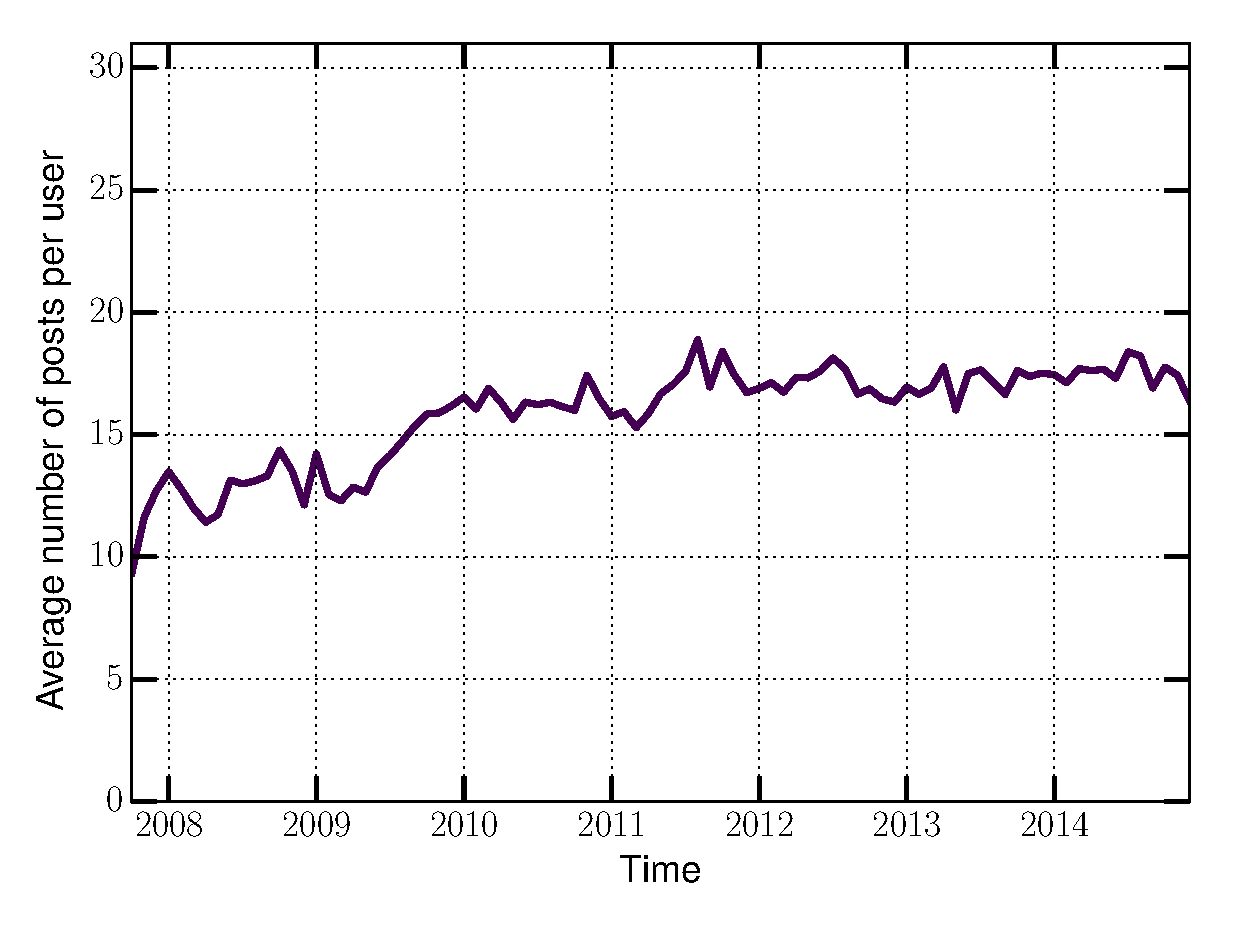
\includegraphics[scale=0.4]{./images/avr_posts_per_user_over_time_total.eps}
\caption{Caption}
\label{fig:avr_posts_per_user_over_time_total}
\end{figure}

\begin{figure}[!tb]
\centering
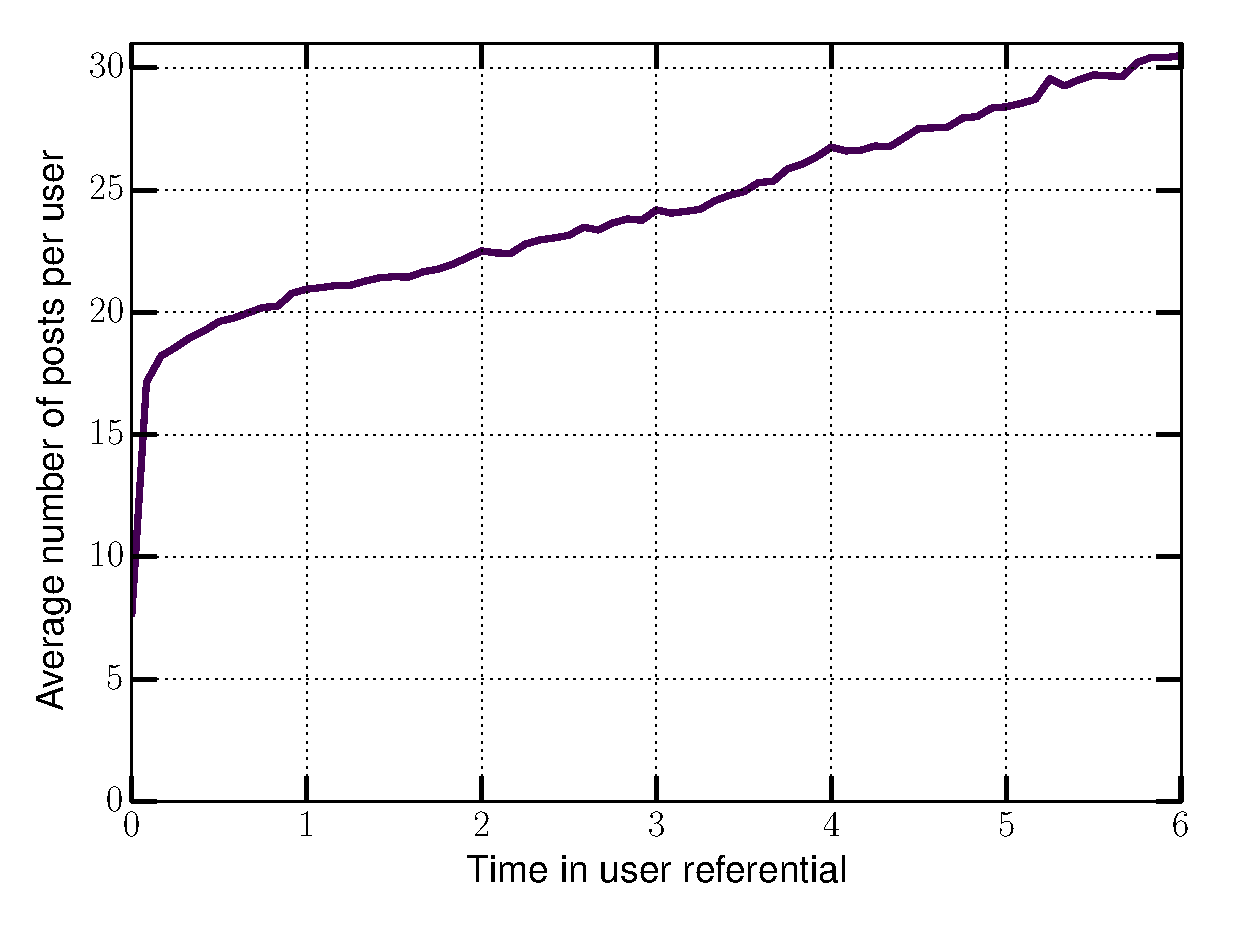
\includegraphics[scale=0.4]{./images/avr_posts_per_user_user_ref_total.eps}
\caption{Caption}
\label{fig:avr_posts_per_user_user_ref_total}
\end{figure}

Figure~\ref{avr_posts_per_user_over_time_total} shows the average number of posts (submissions plus comments) per month by users who were active in that month.  Taken at face value, this suggests that over the first few years of Reddit, users became more active in posting and that per-user activity has remained more or less steady since mid-2011.  

\subsection{Activity relative to a user's lifespan}

%% DC 10: This is the new figure, the one that's adjusted to be relative to user creation date like Figure 5 but aggreated over all users rather than separated by cohort.

%% DC 10: This is my best guess as to what the aggregate version of the avr_posts_per_user_cohorts figure looks like
This average view hides several important aspects of users' activity dynamics.  In Figure~\ref{fig:NEEDED_avr_monthly_active_posts_relative}, we show a different view that emphasizes the trajectory over a user's lifespan.  Here, we scale the x-axis not by clock time, as in the prior figure, but by time since the user's first post: ``1'' on the x-axis refers to one year since the user's account creation, and so on.  
One caution about interpreting the graphs that are relative to the user's start time is that the amount of data available rapidly decreases over time, meaning that values toward the right side of an individual data series are more subject to individual variation.  
%% DC 10: The way to really handle this would probably be confidence intervals, but we should at least note it somewhere and this is the best way I could think of for now.

This figure shows that a user's tenure matters: the longer a user survives, the more posts they make over time.  Interestingly, we see that the curve rises much higher than it does in Figure~\ref{avr_posts_per_user_over_time_total}: users who survive over five years have almost 50\% more posts per year than average. 

\subsection{Cohort-based views of posting activity}

\begin{figure}[!tb]
\centering
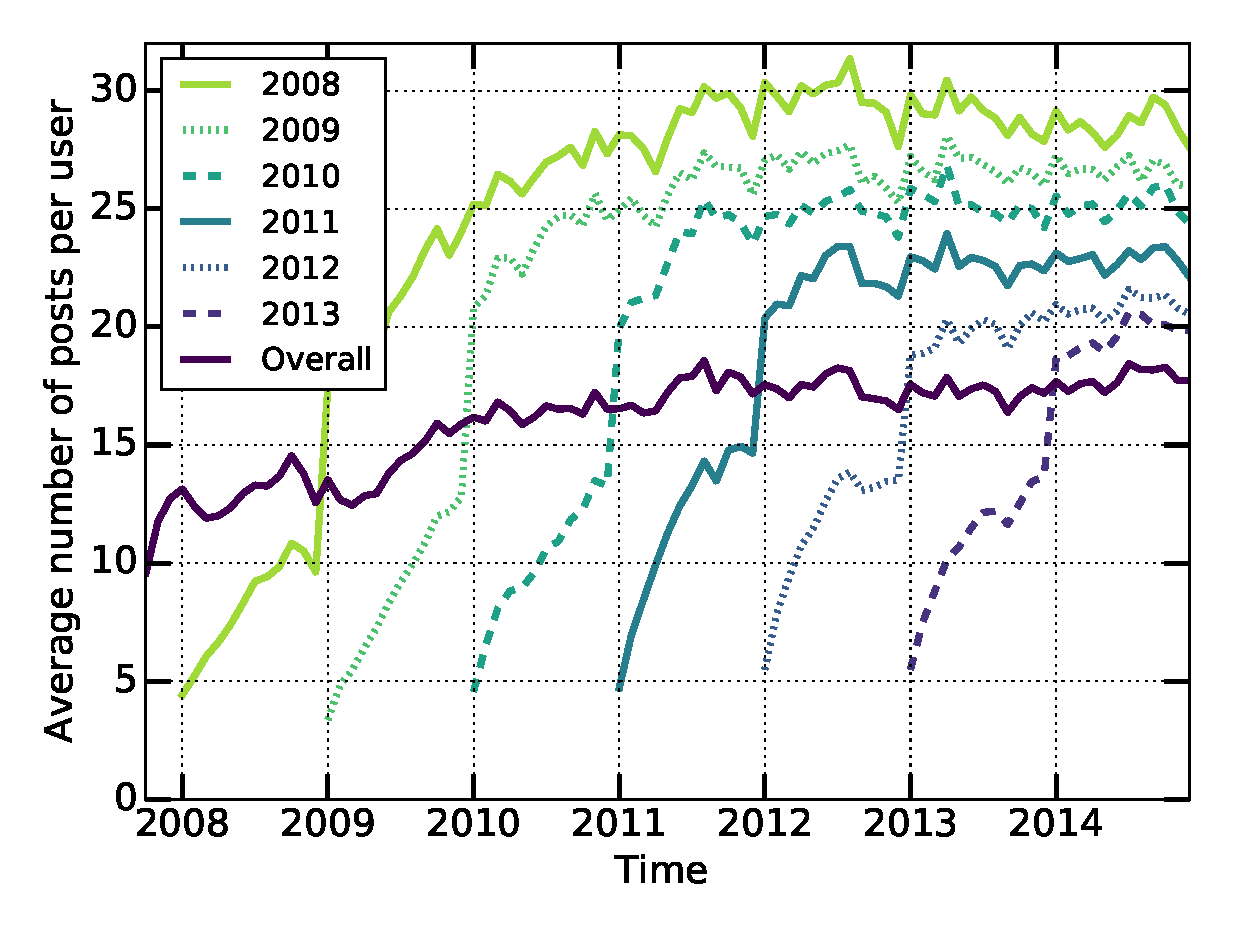
\includegraphics[scale=0.4]{./images/avr_posts_per_user_over_time_cohorts.eps}
\caption{Caption}
\label{fig:avr_posts_per_user_over_time_cohorts}
\end{figure}

Implicitly, the prior figure suggests that older (in the sense of first account activity) users are more active than newer ones, raising the question of whether newer users
are likely to eventually follow in older users' footsteps.  Analyzing users' behavior by cohort, grouping them by account creation year, is one reasonable way to address this question.  Figure~\ref{fig:avr_posts_per_user_over_time_cohorts} shows our first attempt at this analysis.  This figure already shows a significant cohort effect: users from latter cohorts appear to level off at a significantly lower posting average than users from earlier cohorts.  

However, the figure also has an awkward anomaly, the sharp increase in the average number of posts at the end of each cohort's first calendar year in Figure N.  Since we segmented our users by cohorts, by the end of each year onwards, we do not have users joining the network any more and the number of active users does not increase because of new users anymore. This fact, along with the observation that young users tend to post less from Figure~\ref{fig:NEEDED_avr_monthly_active_posts_relative}, drags the average down during the first year, since young users are always coming into the network.  
%% DC 10: A little redundant.  
% This is particularly true for the first month, specially considering that there are many user accounts that are created and only show activity for a single day in reddit, which likely brings the average down.

%% DC 10: I get tired of saying that; it would be useful to define "account creation" as the data handling part earlier as the first visible post in the dataset and just note that they actually created their account earlier than that.

We can largely account for this by still treating users as cohorts based on the year they first posted to reddit, but adjusting the time reference to be relative to the user's first post rather than clock time as we did before.  Figure~\ref{fig:avr_posts_per_user_cohorts_relative} presents this view of the data.

\begin{figure}[!tb]
\centering
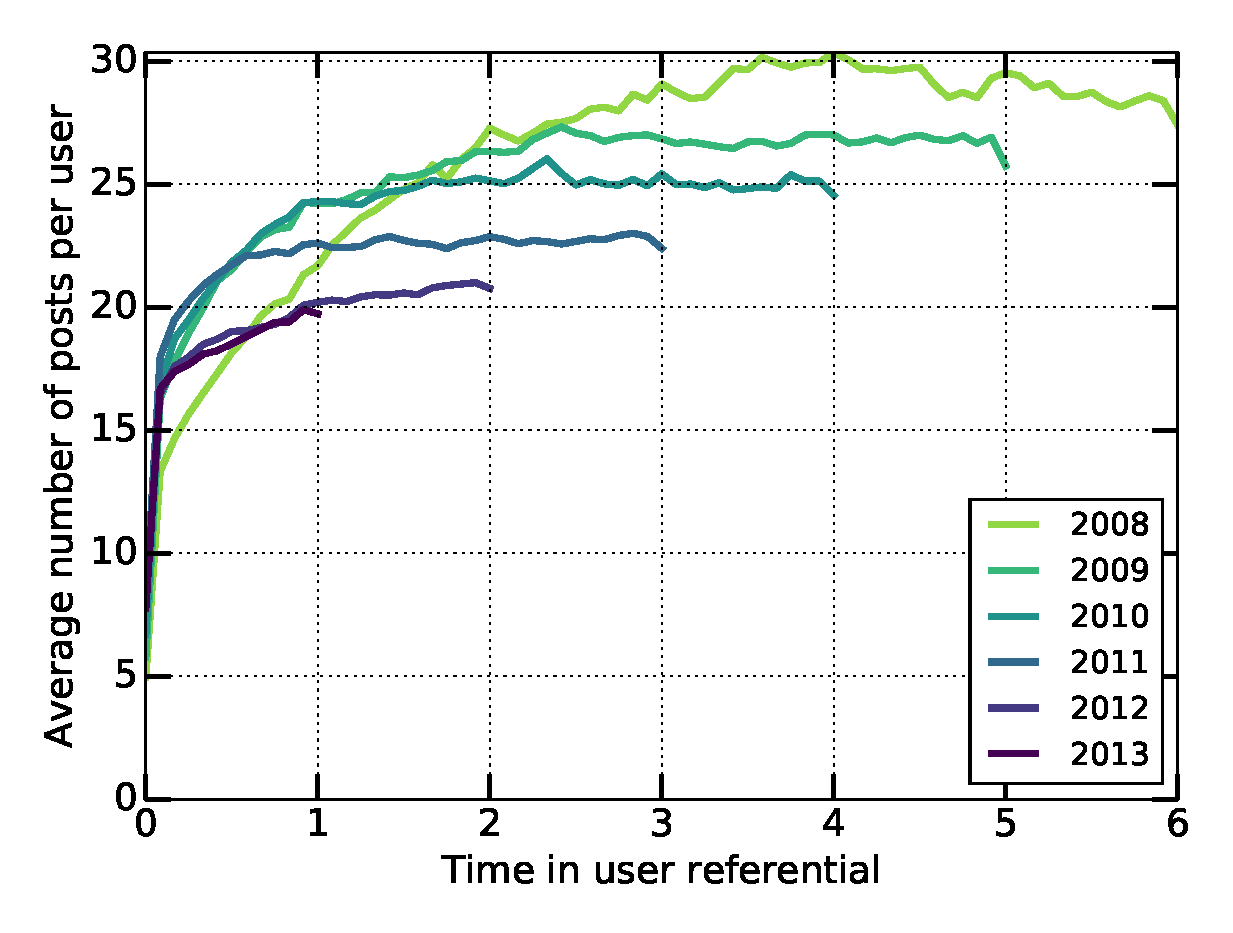
\includegraphics[scale=0.4]{./images/avr_posts_per_user_cohorts.eps}
\caption{Caption}
\label{fig:avr_posts_per_user_cohorts_relative}
\end{figure}

\begin{figure}[!tb]
\centering
\includegraphics[scale=0.2]{./images/avr_posts_per_user_for_surviving_year_for_2008.eps}
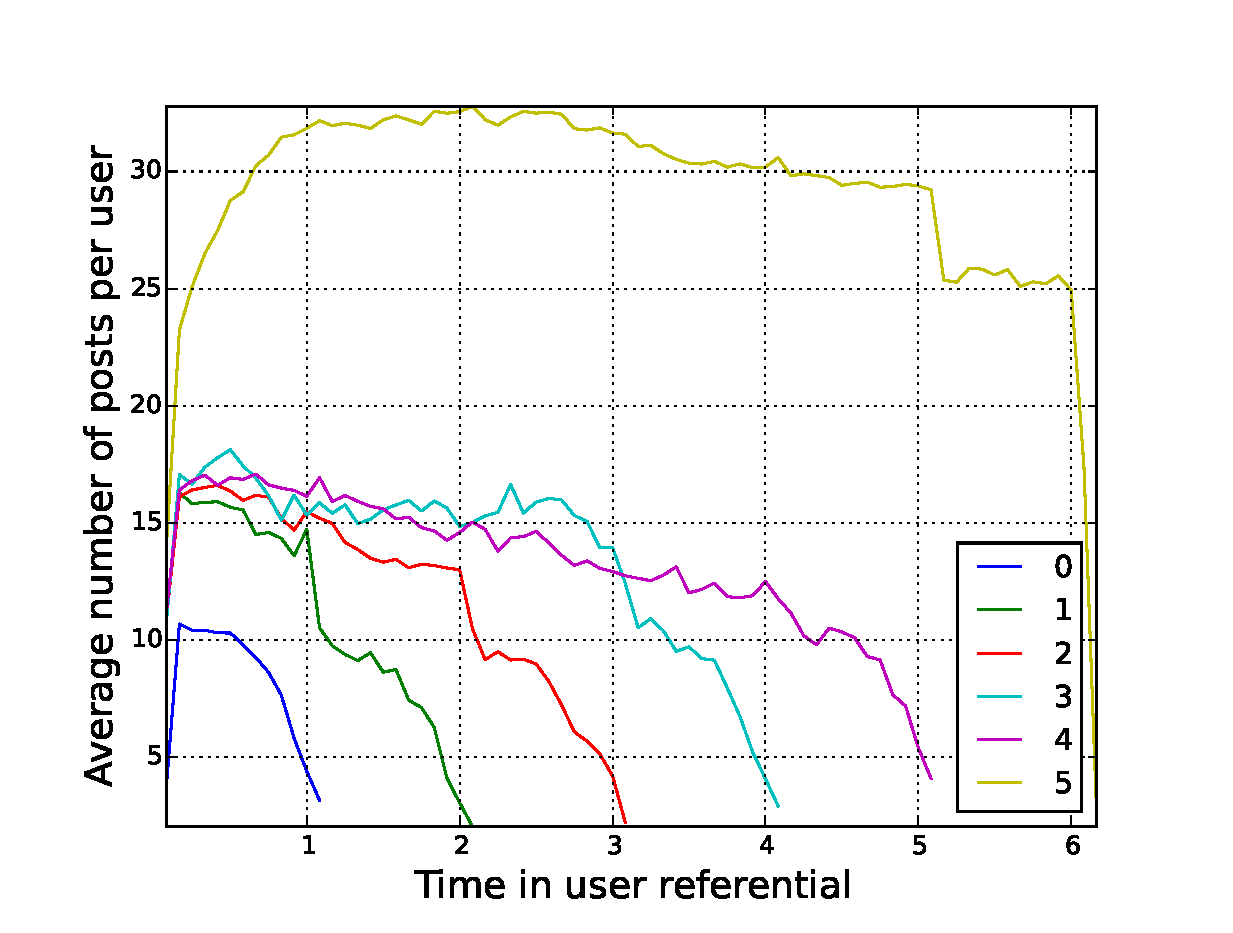
\includegraphics[scale=0.2]{./images/avr_posts_per_user_for_surviving_year_for_2009.eps}
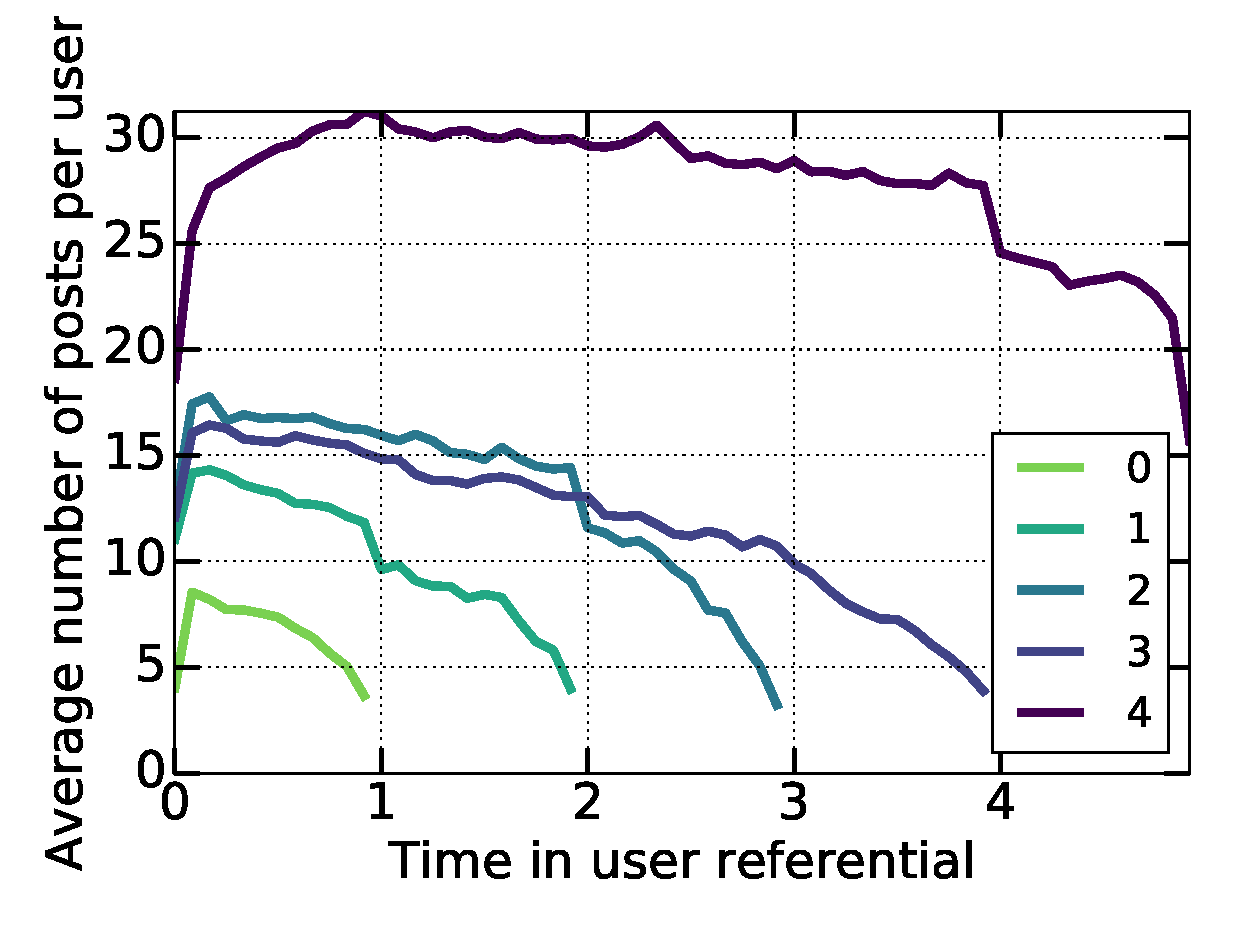
\includegraphics[scale=0.2]{./images/avr_posts_per_user_for_surviving_year_for_2010.eps}
\includegraphics[scale=0.2]{./images/avr_posts_per_user_for_surviving_year_for_2011.eps}
\includegraphics[scale=0.2]{./images/avr_posts_per_user_for_surviving_year_for_2012.eps}
\includegraphics[scale=0.2]{./images/avr_posts_per_user_for_surviving_year_for_2013.eps}
\caption{Caption}
\label{fig:avr_posts_per_user_for_surviving_year}
\end{figure}

%% DC 10: Part of me would be curious about either an inset for the first three months, and/or a log-2 scale for time where the first year gets half the frame, etc.  My guess is that the log scale is hard to read because it's an unusual way to present time, but it does have an advantage in that most of the data is on the "left" of the graph and that would emphasize attention toward it, maybe.
This figure suggests that there may not be strong cohort effects early in a user's lifespan, although even after six months users in the most recent 2012 and 2013 cohorts appear to be less active than those in earlier groups.  In the long run, however, a striking pattern emerges: different cohorts stabilize in different levels of behavior, and in particular, the steady state activity for surviving users goes down for every year from 2008 to 2012.  

This raises interesting questions of why we see this behavior.  One plausible explanation is that users who find a community early in its life are also more likely than average to be those who will be attracted to it, in the same way that early ratings for a movie in a recommender system are likely to be higher than later ratings because the people who are most attuned to the movie are likely to see it earlier \cite{if_we_can_find_one}.  Another is an argument based on cumulative advantage, status, and attention-seeking: surviving users from earlier cohorts might be more capable of producing content that gets attention from other users.  This would lead to them getting more comments and votes for their content, and people who get positive attention are more likely to return \cite{joyce-kraut, wikipedia, everything2_papers}.  

We're not taking a position on either of these as the mechanism that explains these results; both would be interesting avenues for future work.  We do suggest that looking at Reddit from a cohort and user-based view rather than an aggregate community view helped us uncover interesting phenomena and questions that would have been invisible to more commonly-performed analyses of community behavior. 

%% DC 10: The status bit is intriguing but needs to be explained a little better.  Took a little shot at it but framing it in terms of cumulative advantage rather than status
%% DC 10:This, too, would need to be explained/justified/supported, and I can't come up with a plausible one, so deleting it.
%Yet another explanation would be that earlier users demographics were different in terms of age and interests, for example, and these correlate to the fact that they present a higher activity.

%% DC 10: There is a mysterious question about why 2008 ramps up more slowly, that I would interpret in the "there was less to comment on" framing that we've chatted about before.  You could actually do an analysis to test this, where for each user, the number of posts in a month is normalized by the number of posts made in reddit in that month: that is, how active is the user relative to the total amount of activity in reddit.  This is _not_ a linear scaling when the analysis is relative to the user's initial start date, and I would be curious to see what it showed.


%%%% DanCo stopping here %%%%

%% DC 10: These are actually a separate section, or sections, for me.  In particular, Users' Effort and the Simpson almost certainly need to be combined.  

\subsection{Users' Effort}

In addition to the raw number of posts, comments length can also be considered as a proxy for user effort in the network. Users that type more put more of their time in the network, contribute with more content and might create stronger ties with the community. The Figure N shows the evolution of the monthly average comment length in reddit.

\begin{figure}[!tb]
\centering
\includegraphics[scale=0.4]{./images/avr_comment_size_over_time_total.eps}
\caption{Caption}
\label{fig:avr_comment_size_over_time_total}
\end{figure}

\begin{figure}[!tb]
\centering
\includegraphics[scale=0.4]{./images/avr_comment_size_user_ref_total.eps}
\caption{Caption}
\label{fig:avr_comment_size_user_ref_total}
\end{figure}

Based on the downwards tendency of the comment length, one could possibly imagine that the user commitment with the network is lowering over time. This, however, might not be the best way to interpret this information. Figure N shows the comment length per cohort based on the user referential time. This figure shows that, unlike the average overall network comment length, surviving users increase the size of their contributions to the community over time. This is true for all users cohorts. The important thing to notice here is that, while user comments get longer as they stay for longer in the network, younger users start from a lower baseline comment than older users. Together with the fact that recent reddit has experienced exponential-like growth, the heavier weight when evaluating the averages for Figure N as the years go by is shifted towards the size of the ever growing younger generation, and this younger generation brings the average down since they start writing less.

Some possible explanations for this difference in the starting points could be that older users are, again, sampled from a different demographics that is more committed and willing to spend more effort into developing their virtual identity. Also, it could be that it is a natural evolution of the community, as older users have taken most of the main space of interests when it comes to creating new subreddits and starting these communities, new users have it all already made and sometimes might feel intimidated or not motivated to create new topics or communities that already exist or that are less likely to compete with the existing ones. In a way, these new users could behave more as lurkers, while the older users are the ones that laid the foundation of reddit.

\begin{figure}[!tb]
\centering
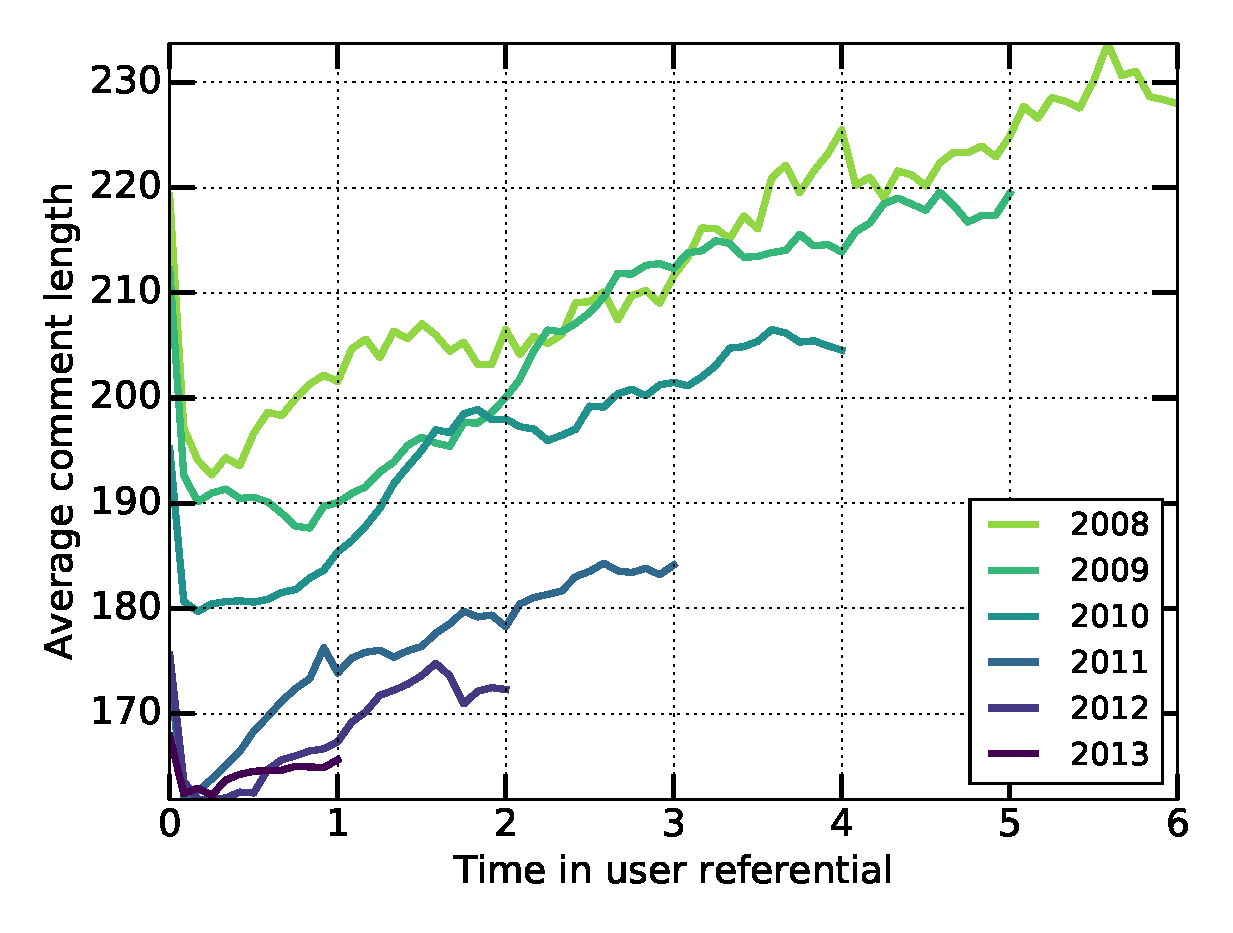
\includegraphics[scale=0.4]{./images/avr_comment_size_cohorts.eps}
\caption{Caption}
\label{fig:fig_label}
\end{figure}

\begin{figure}[!tb]
\centering
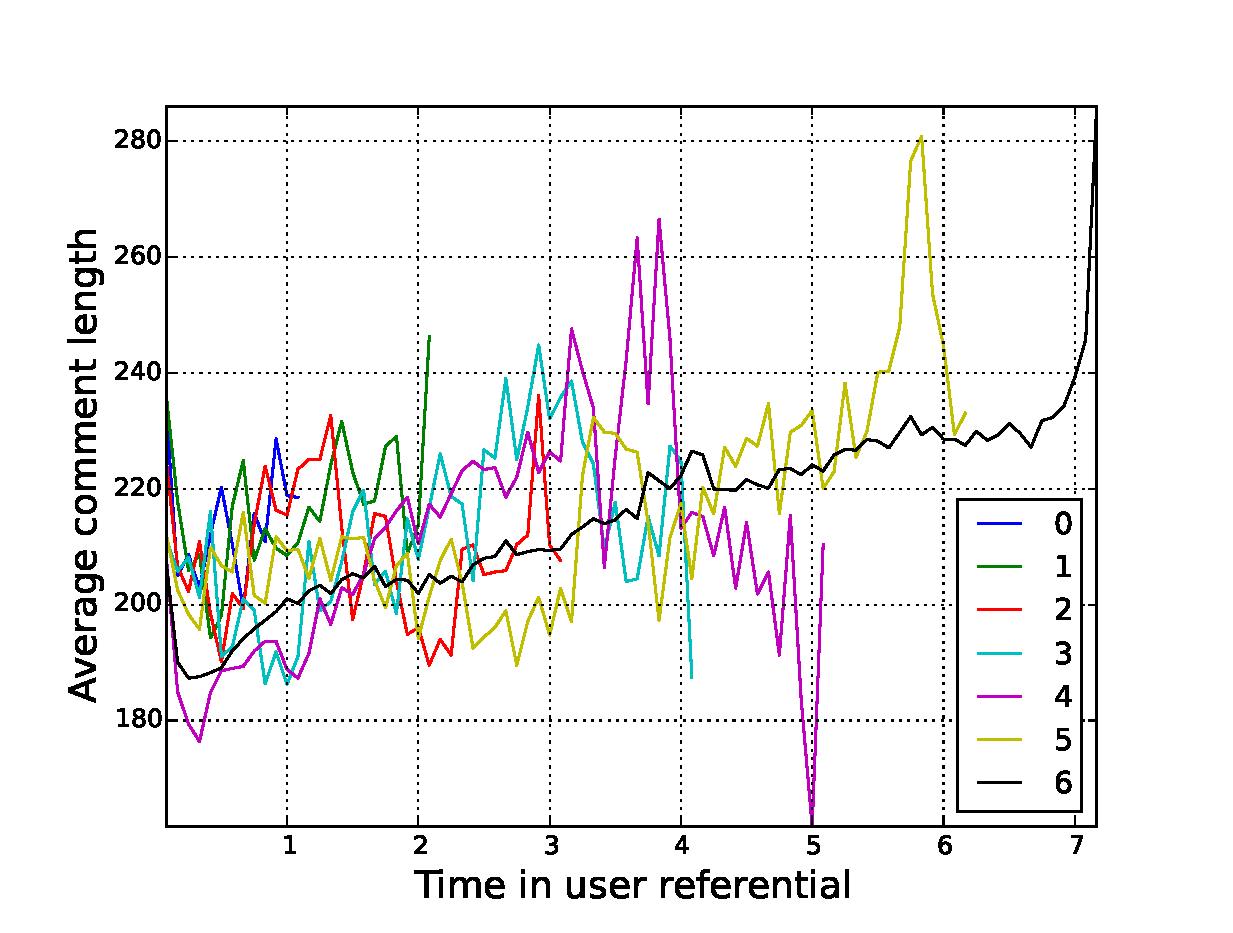
\includegraphics[scale=0.2]{./images/avr_comment_length_for_surviving_year_for_2008.eps}
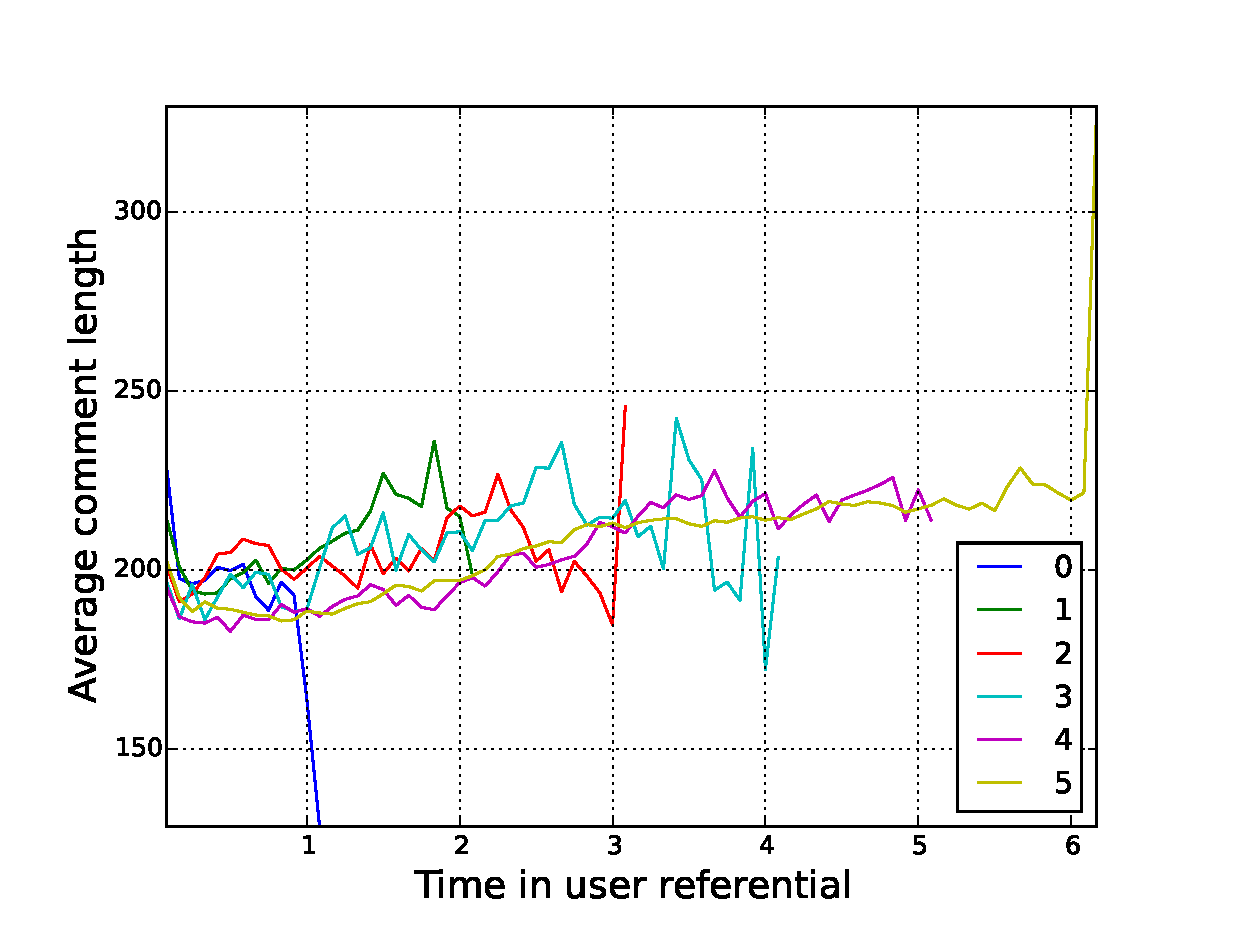
\includegraphics[scale=0.2]{./images/avr_comment_length_for_surviving_year_for_2009.eps}
\includegraphics[scale=0.2]{./images/avr_comment_length_for_surviving_year_for_2010.eps}
\includegraphics[scale=0.2]{./images/avr_comment_length_for_surviving_year_for_2011.eps}
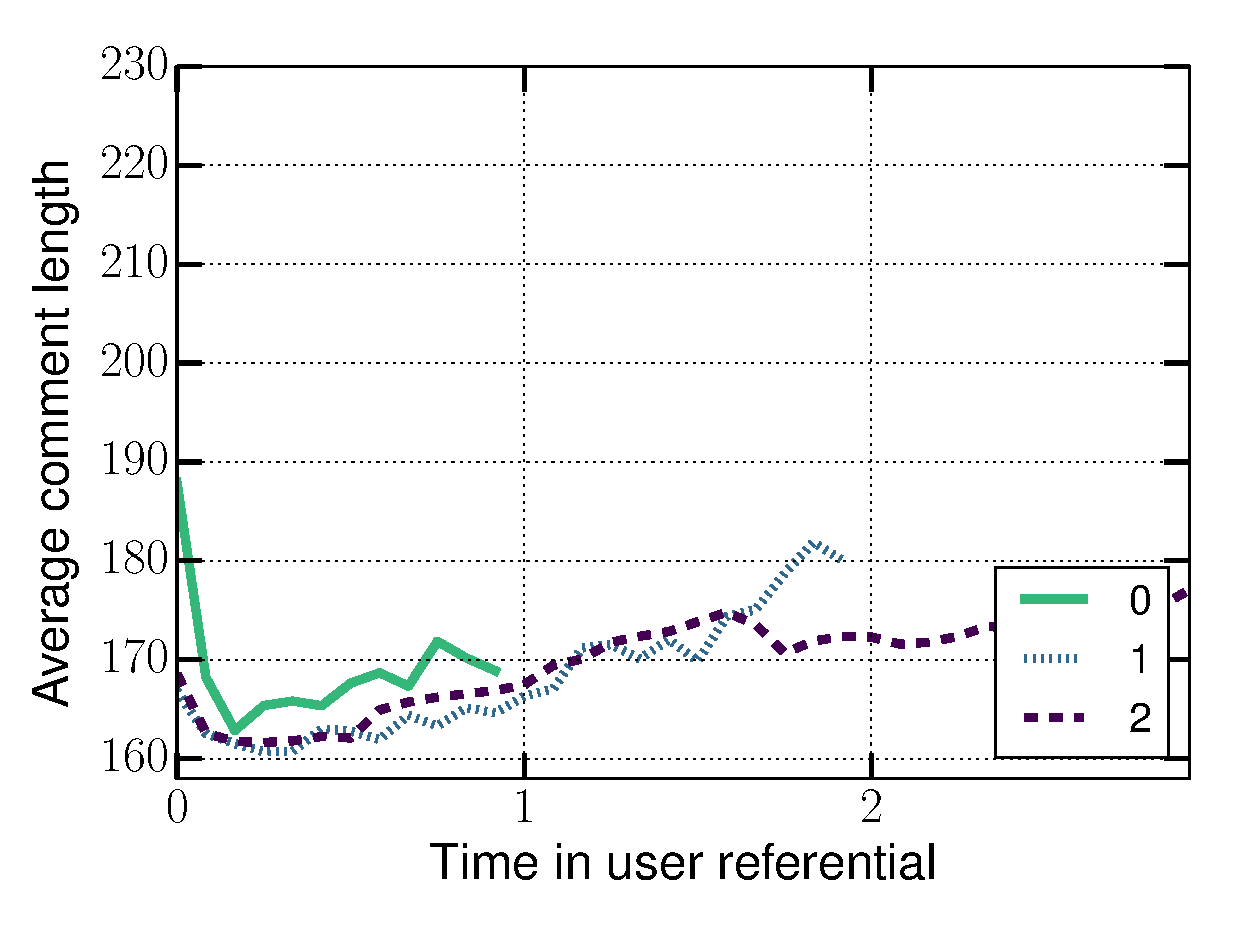
\includegraphics[scale=0.2]{./images/avr_comment_length_for_surviving_year_for_2012.eps}
\includegraphics[scale=0.2]{./images/avr_comment_length_for_surviving_year_for_2013.eps}
\caption{Caption}
\label{fig:avr_comment_length_for_surviving_year}
\end{figure}

Yet another hypothesis that we might consider is that users are lowering their activity due to an ``initial value problem''. We can imagine that users, as they join the network, they tend to produce content according to the norms of what they see. If we look at the cohort posting size over time superimposed with the average size for the whole network, we can see that the starting point of each cohort seems to agree to a reasonable extent to the average over the total network. This way, users would be simply reproducing things as they see in their early months, but as we have seen in Figure N, users start their life posting longer content, but there is a strong decrease in size for the early months before the size increases for the surviving users.

\begin{figure}[!tb]
\centering
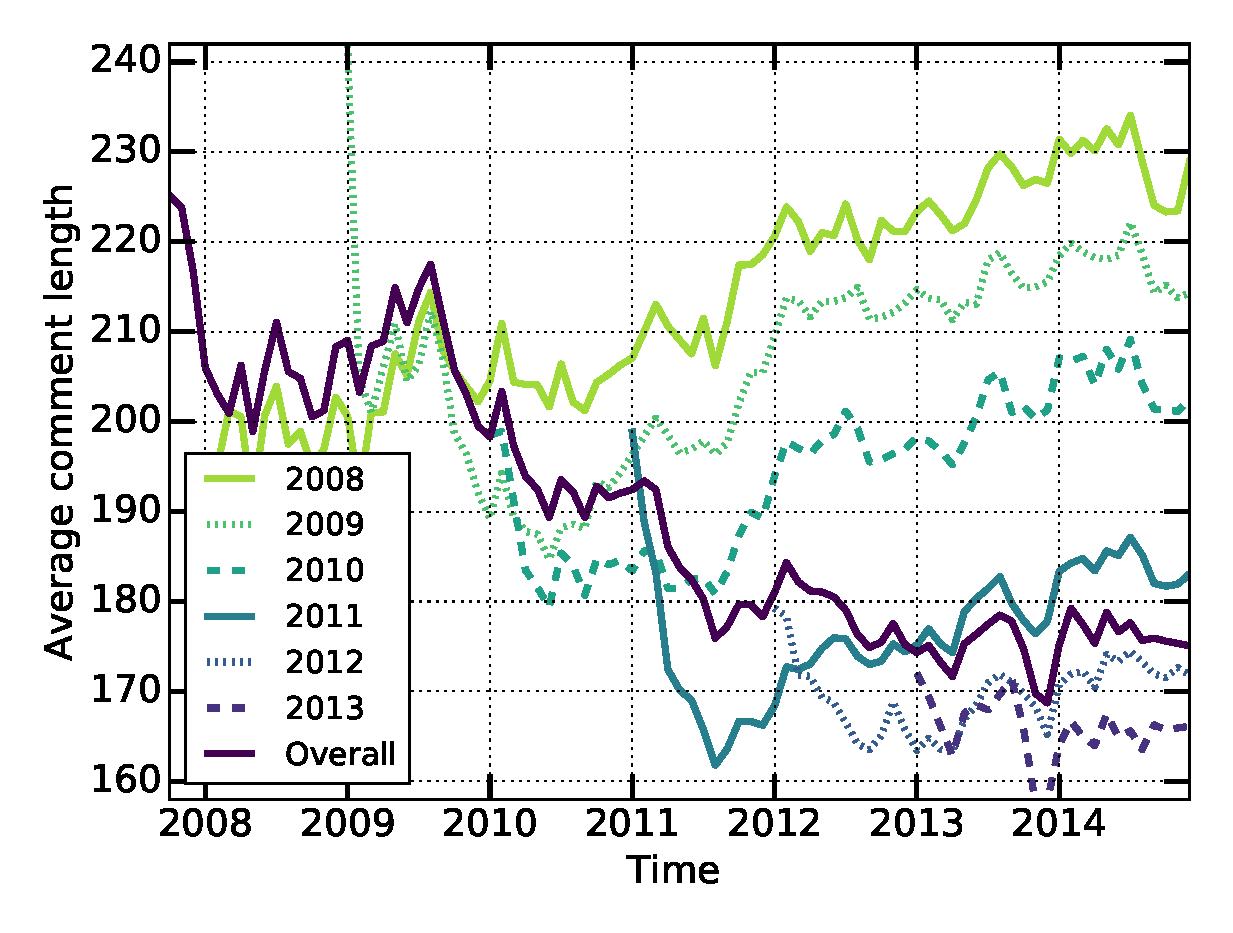
\includegraphics[scale=0.4]{./images/avr_comment_size_over_time_cohorts.eps}
\caption{Caption}
\label{fig:fig_label}
\end{figure}

\subsection{Activity Nature}

One common question from the literature is what sorts of activities users engage in; this can be used as a metric of community health (cites) or to categorize users into roles they play in the community (cite).  In reddit, we do not have per-user voting behavior, but we do have the number of comments and submissions, and a naive view of this would look at the ratio of comments to submissions over time.

While submissions can be considered new content that an author generates, a comment can be considered as a contribution to an existing content from another author. Since the total number of comments always surpasses the number of submissions, Figure N shows the evolution of the ratio of comments per submission over time for users created from 2008 until 2013. It is important to highlight here that we are not talking about the average number of comments a submission gets, but how many comments a user authors for each of his/her submissions.

\begin{figure}[!tb]
\centering
\includegraphics[scale=0.4]{./images/comments_per_submissions_over_time_total.eps}
\caption{Caption}
\label{fig:comments_per_submissions_over_time_total}
\end{figure}

\begin{figure}[!tb]
\centering
\includegraphics[scale=0.4]{./images/comments_per_submissions_user_ref_total.eps}
\caption{Caption}
\label{fig:comments_per_submissions_user_ref_total}
\end{figure}

We have found that segmenting users and subreddits by cohorts on the years that of the first comment highlights significant differences of behavior and help us to understand how reddit changed over these years.


Table 1: Number of distinct users that authored comments and submissions segmented by the year of the first post of the user. The Total numbers are based on posting data from 2007 until 2014, corresponding to our full dataset. The Oct 1st, 2014 onwards numbers are based on the last 3 months of data we have, and we consider this as the current, active reddit.


Table 2: Number of distinct subreddits segmented by the year of the first post of the user. The Total numbers are based on posting data from 2007 until 2014, corresponding to our full dataset. The Oct 1st, 2014 onwards numbers are based on the last 3 months of data we have, and we consider this as the current, active reddit.

Table indicates that reddit grew significantly from 2007 until 2012, practically doubling the number of new users per year for each of these years, with similarly significant growth in subreddits. Although the most expansive growth happened in the first years, more than half of the registered users are from the last 2 years, and their behavior is significantly different than previous users, impacting in the overall behavior of the community. For instance, users from the 2014 cohort have a higher tendency to make submissions instead of comments, in contrast with all the previous cohorts.

Looking at the user time referential, the evolution of the number of comments per submission shows a decreasing trend for the older cohorts. One explanation for this is that, as the community grew, more content from an absolute point of view was present in the social network, and therefore users had more reason to make contributions commenting instead of submitting new content that was likely to already exist.

%% DC 10: This needs to be managed better, somehow; right now it's a little overwhelming as a blob of graphs.  It might be better to pick one representative year rather than present them all.  Also, this might an excellent place to introduce (or reintroduce) the point that when you zero-adjust, you have less and less data off to the right; the abrupt jumps that especially the later years (4, 5, 6) from the earlier cohorts show at the end are almost surely driven by low n users, right?
\begin{figure}[!tb]
\centering
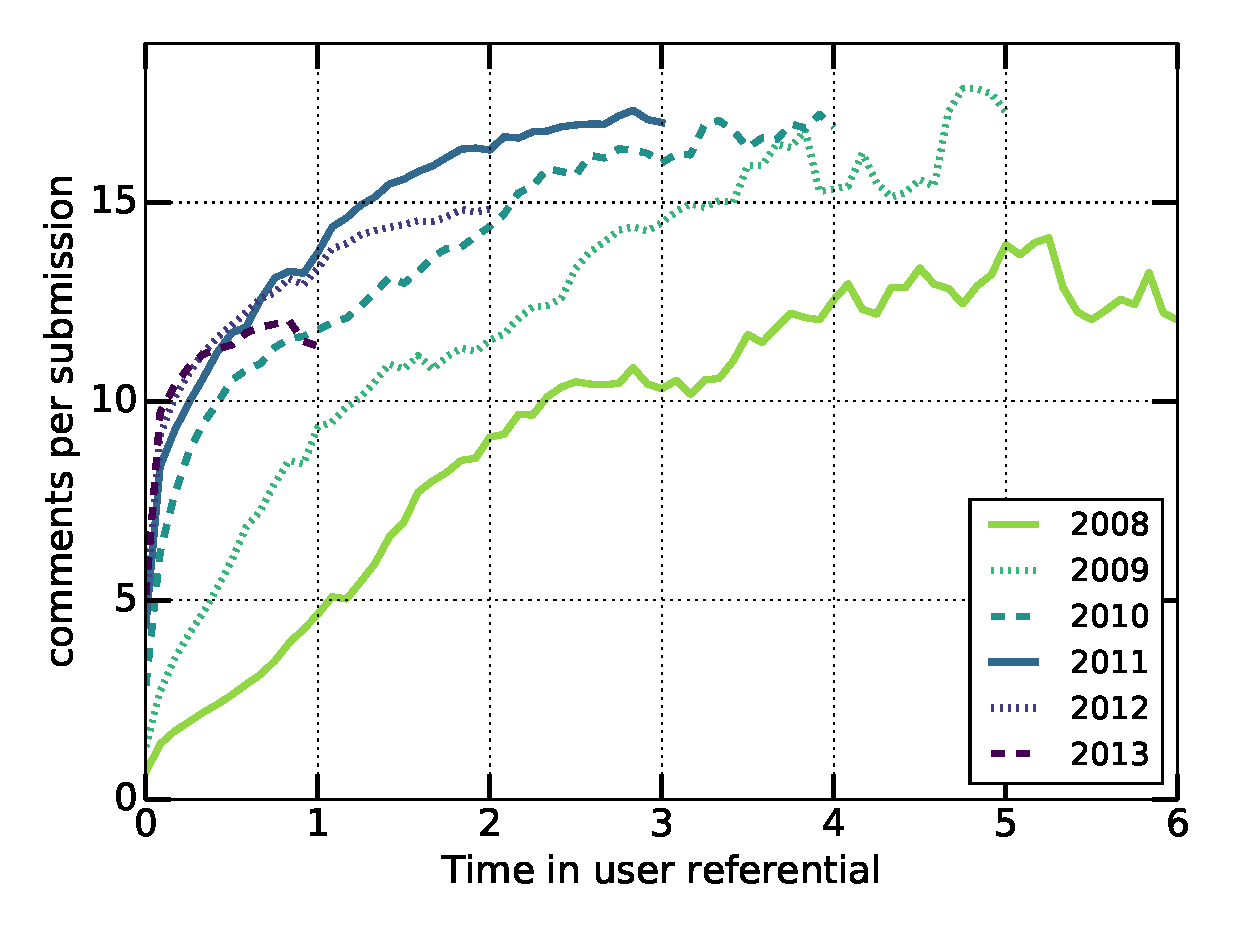
\includegraphics[scale=0.4]{./images/comments_per_submissions_cohorts.eps}
\caption{Caption}
\label{fig:comments_per_submissions_cohorts}
\end{figure}

\begin{figure}[!tb]
\centering
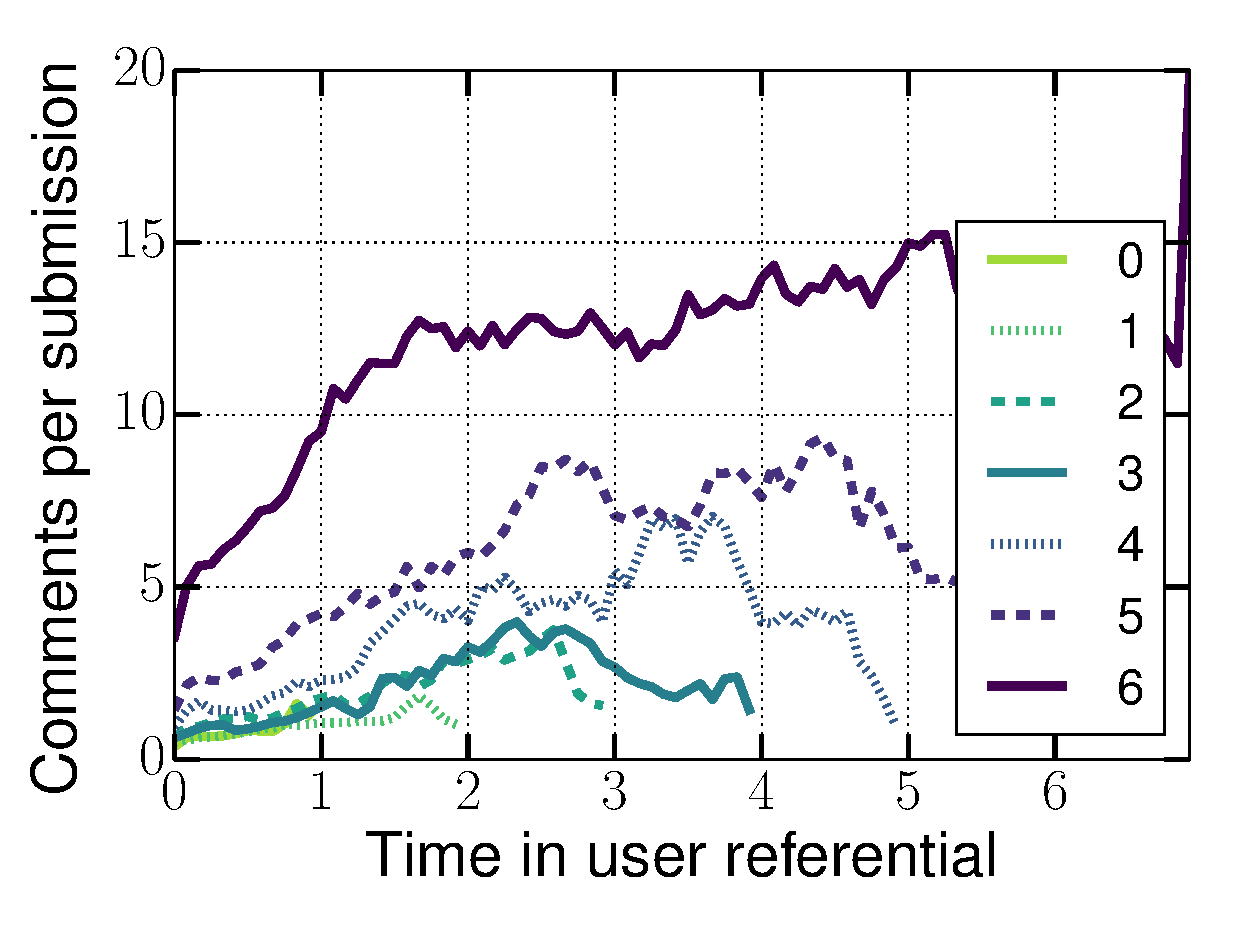
\includegraphics[scale=0.2]{./images/comments_per_submissions_for_surviving_year_for_2008.eps}
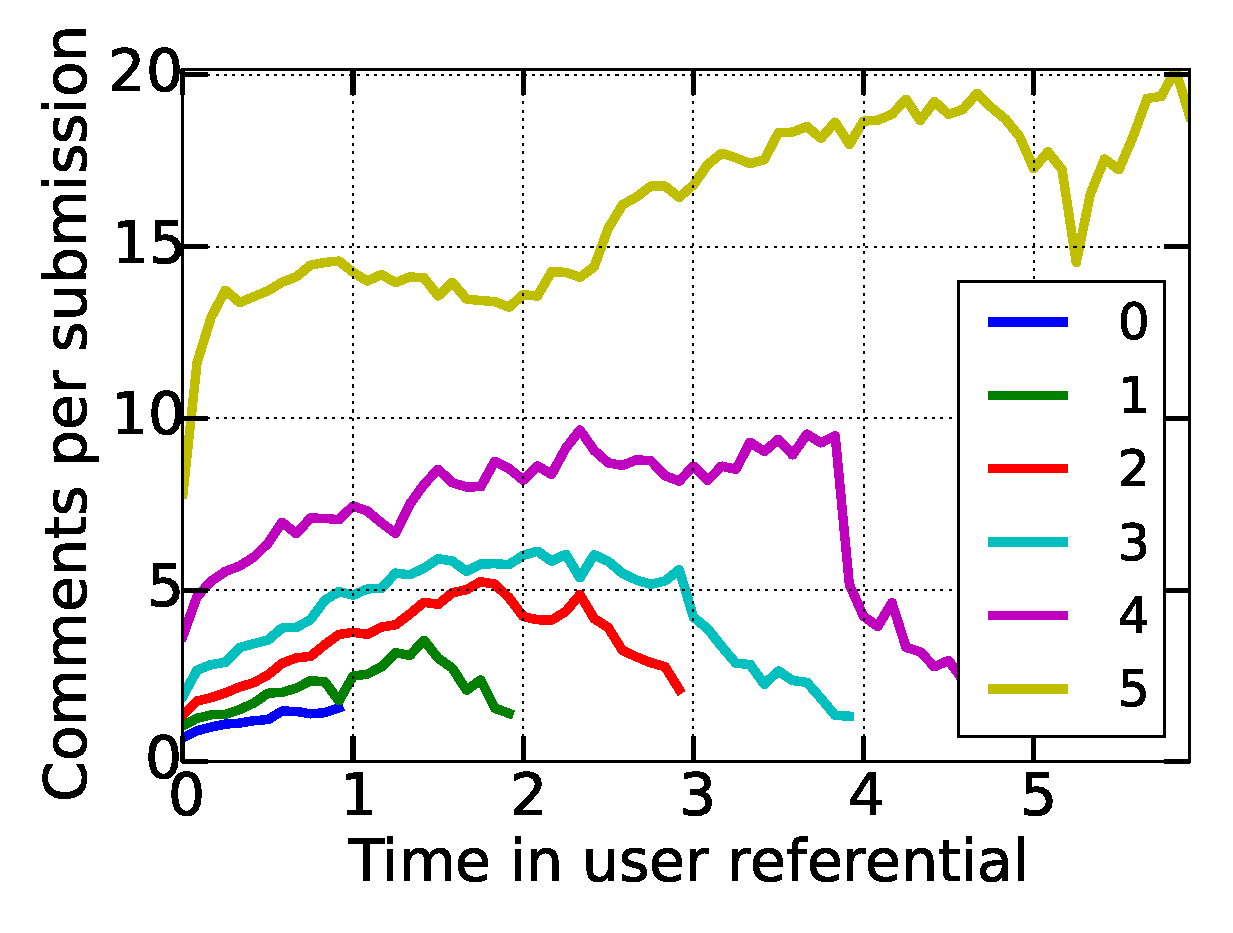
\includegraphics[scale=0.2]{./images/comments_per_submissions_for_surviving_year_for_2009.eps}
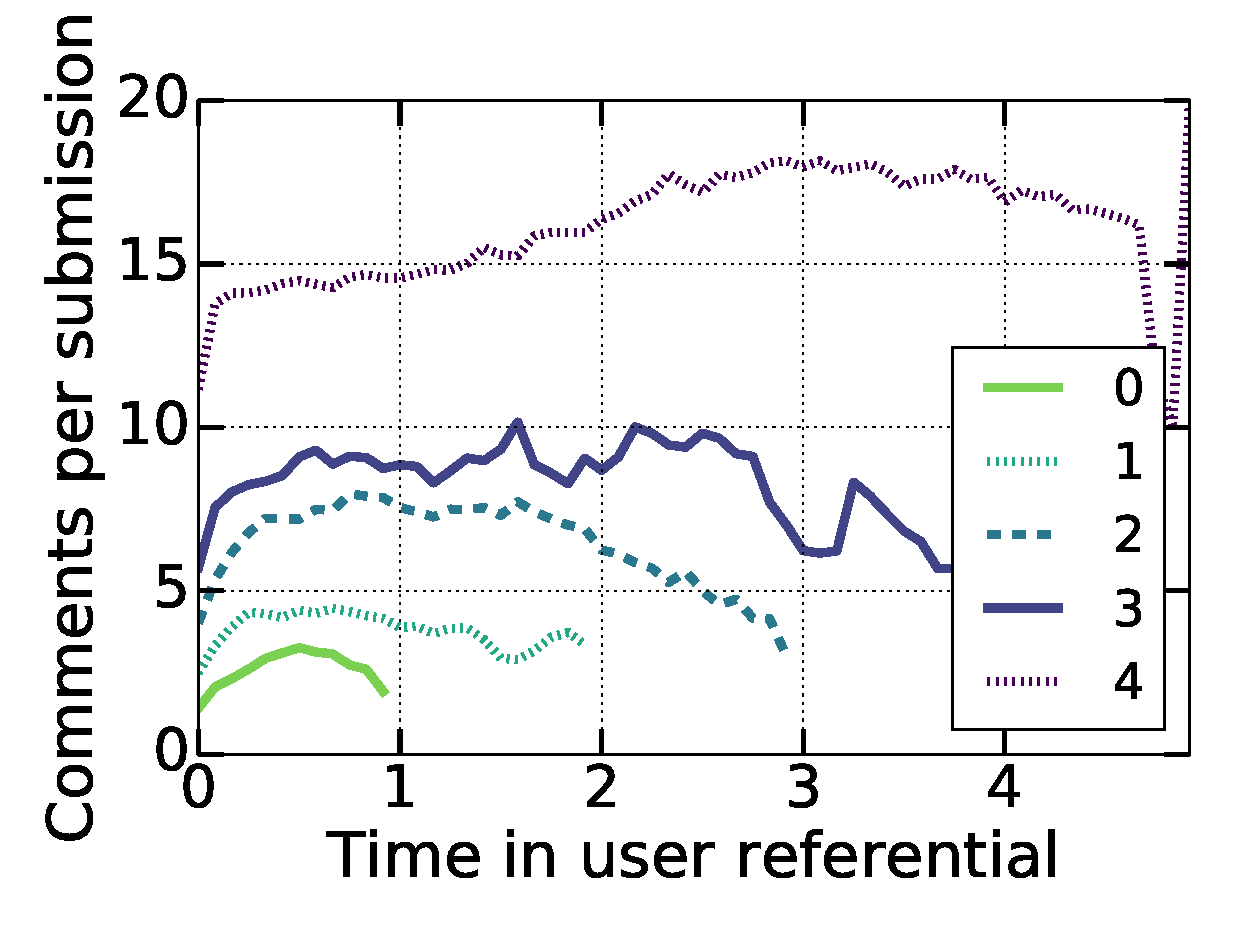
\includegraphics[scale=0.2]{./images/comments_per_submissions_for_surviving_year_for_2010.eps}
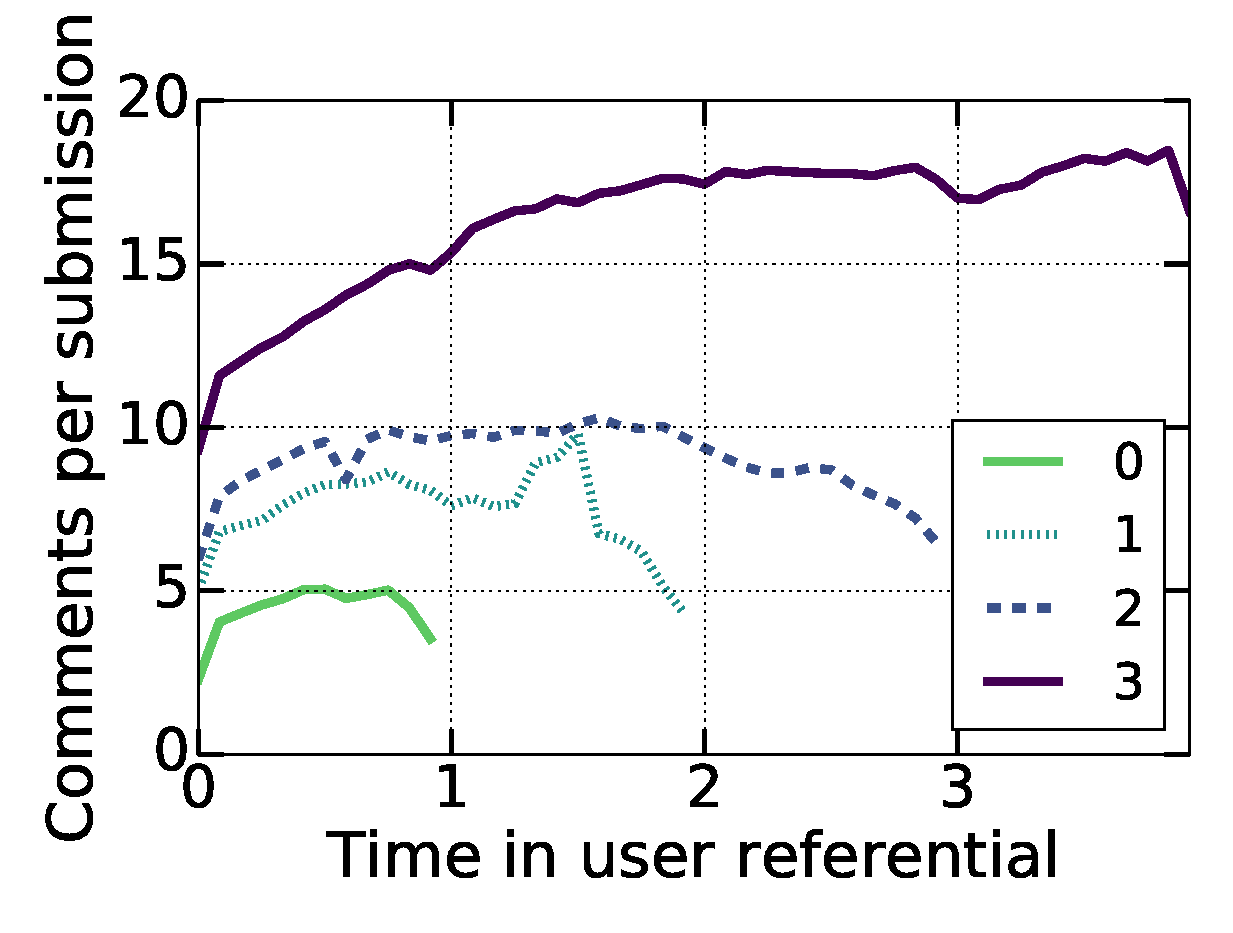
\includegraphics[scale=0.2]{./images/comments_per_submissions_for_surviving_year_for_2011.eps}
\includegraphics[scale=0.2]{./images/comments_per_submissions_for_surviving_year_for_2012.eps}
\includegraphics[scale=0.2]{./images/comments_per_submissions_for_surviving_year_for_2013.eps}
\caption{Caption}
\label{fig:comments_per_submissions_for_surviving_year}
\end{figure}

\subsection{Users' Survival}

The simplest definition of an active user in reddit is to set a threshold date and define that every user that posted after that date is an active user and users that do not show any kind of behavior are ``dead''. This, however, is a limited interpretation of how users decide to stay or leave the network, specially if we want to analyse how this behavior changed over time. Also, since our users might always come back to the network at a later time, they might be ``reborn'', that means we have right censored data.

To account for these, we look at a one year window of time for each user. This way, we avoid the right censored data and the possibility that a user might have come back to the network at a later time. Given this, we segment users by their cohort and define that users active in the last 3 months of this one year window are active users. Based on this data manipulation, we present the Kaplan-Meier (cite) survival curve in Figure N.

\begin{figure}[!tb]
\centering
\includegraphics[scale=0.4]{./images/kaplan_meier_users.eps}
\caption{Kaplan-Meier estimator for one year of posting behavior for each user. Users for which the last posting day was in the first nine months of the one year window are considered ``dead''. This graph shows the percentage of surviving users per number of days since it first posted segmented by the cohort year the user joined the network.}
\label{fig:kaplan_meier_users}
\end{figure}

As previously mentioned, reddit shows a significant number of ``single time users'' that only post once in their existence. This can be seen in the initial drop in the first day. An interesting thing to see is that, although different cohorts level in different survival values, the ``user decay'' is similar throughout all of them. Not only that, but there is a general trend for older cohorts to die faster than younger ones. One possible explanation for that is that early reddit still lacked in content, with few subreddits to submit and few submissions to comment. This could lead to a higher number of users that did not stayed around after their initial impressions. 

\begin{figure}[!tb]
\centering
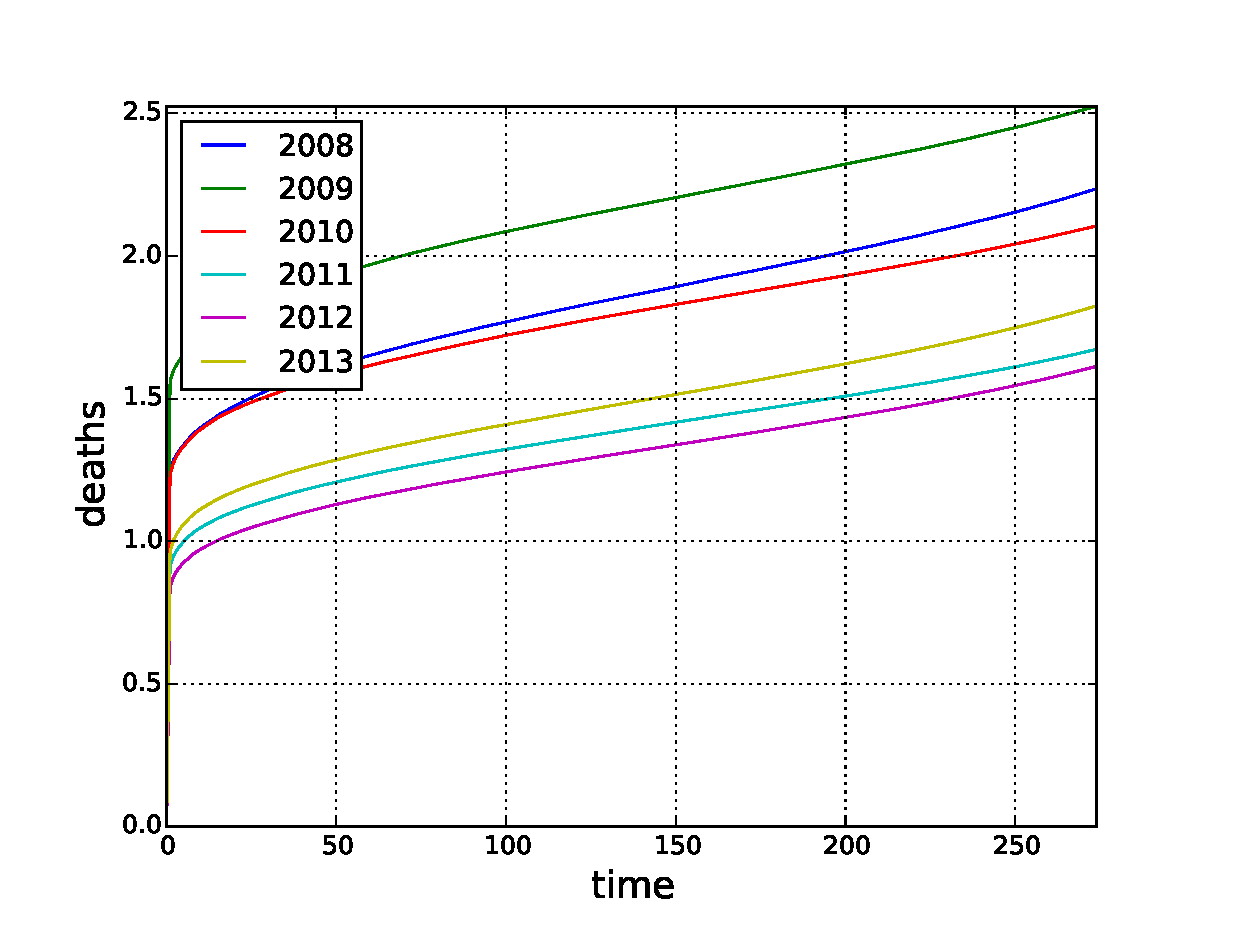
\includegraphics[scale=0.4]{./images/nelson_aalen_users.eps}
\caption{Caption}
\label{fig:nelson_aalen_users}
\end{figure}
